% !TeX program = pdflatex
% =============================================================================
% Aufgabenblatt 1: Gewichtskraft & Federkraft
% UZH Praktikum I -- Sara Romer Urban, Kantonsschule im Lee, HS2026
% Klasse: 2e (26.08.2026)
%
% Beginnt mit einer Ziel-Box (was in dieser Lernaufgabe untersucht wird,
% ohne das Ergebnis vorwegzunehmen) und enthaelt die Federkraftmesser-
% Lernaufgabe (Stationsexperiment mit Excel-Vorlage, analog zur
% PhET-Lernaufgabe bei Kondensatoren), eroeffnet durch ein Kraeftediagramm
% (LZ6, Aufwaermuebung als erste Frage der Lernaufgabe selbst): die SuS
% messen an zwei Federn (eine staerkere Feder, eine Federwaage)
% Gewichtskraft (mit dem exakten g=9.81 N/kg, nicht gerundet) gegen
% Laengenaenderung, tragen die Werte in
% gewichtskraft-federkraft-messvorlage.xlsx ein und leiten daraus
% F=D*Delta x sowie D selbst her (LZ5), inkl. Umrechnung der eigenen
% D-Werte nach N/m von Hand (Teil 1b). Teil 2b und Teil 3b sind als
% Transferaufgaben angelegt: aus der unkalibrierten Feder mit Stift, Massen
% und Gehaeuse selbst eine Federwaage bauen (2b), dann ueberlegen, was sich
% am Vorgehen fuer eine Mond-Federwaage aendern muesste (3b) -- Aufgaben,
% die eine Excel-Vorlage brauchen, gehoeren ins Aufgabenblatt, unabhaengig
% vom Zeitpunkt der Bearbeitung. Lernziele, Einleitung, Theorie und alles
% im Plenum Behandelte stehen in
% arbeitsblatt2-gewichtskraft-federkraft-teil1.tex; die generische
% Umrechnung N/cm->N/m an vorgegebenen Werten steht dort in
% gewichtskraft-federkraft-zusatzaufgaben.tex.
%
% Quellen: lernziele.md (dieser Ordner), gewichtskraft-federkraft-notizen-
% sara-romer.txt (Besprechungsnotizen von Sara Romer), gewichtskraft-
% federkraft-lektionsplan.tex (freigegebene Diskussionsgrundlage, dieser
% Ordner), Bilder/Federkonstante_Messung_setup.jpg (Foto des Stationsaufbaus).
% =============================================================================
\documentclass[addpoints,11pt,a4paper]{exam}

\usepackage[T1]{fontenc}
\usepackage[utf8]{inputenc}
\usepackage[ngerman]{babel}
\usepackage{lmodern}
\usepackage[a4paper,margin=2.2cm,headheight=14pt]{geometry}
\usepackage{amsmath}
\usepackage{siunitx}
% Hausstil: zusammengesetzte Einheiten immer als echter Bruch (\frac), nicht
% als Inline-Schrägstrich oder \tfrac -- gilt global für jedes \si/\SI.
\sisetup{per-mode=fraction,fraction-command=\frac}
\usepackage{array,booktabs,tabularx,multirow}
\usepackage{enumitem}
\usepackage{xcolor}
\usepackage{colortbl}
\usepackage{tikz}
\usepackage{physics}
\usepackage[most]{tcolorbox}
\usepackage{lastpage}
\usepackage{graphicx}
\usepackage{hyperref}

\usetikzlibrary{arrows.meta,calc,angles,quotes,decorations.pathmorphing}

\usepackage{setspace}
\usepackage{needspace}
\setlength{\parindent}{0pt}
\setlength{\parskip}{0.6em}
\setstretch{1.08}
\setlist[itemize]{itemsep=0.4em}

% -----------------------------
% Farben (Corporate-Farbschema Physik KFR)
% -----------------------------
\definecolor{titleblue}{HTML}{183A6B}
\definecolor{accentblue}{HTML}{2E6F9E}
\definecolor{lightblue}{HTML}{EAF4FB}
\definecolor{verylightblue}{HTML}{F7FBFE}
\definecolor{lightgray}{HTML}{F4F6F8}
\definecolor{darkgray}{HTML}{4A4A4A}
\definecolor{accentorange}{HTML}{D9720C}
\definecolor{accentpurple}{HTML}{7B2D8E}
% Theorie-Block: eigene Farbe (grün).
\definecolor{theorygreen}{HTML}{2E7D4F}
\definecolor{lighttheorygreen}{HTML}{EAF7EF}
% Gruppenarbeit-Box: eigene Farbe (Petrol/Teal).
\definecolor{groupteal}{HTML}{1B7F72}
\definecolor{lightgroupteal}{HTML}{E8F5F3}
% Hinweisbox: Orange (accentorange), für wichtige Klarstellungen.
\definecolor{lightorange}{HTML}{FCEEE0}
% Formelbox: Violett (accentpurple), für die zentralen Formeln dieser Einheit.
\definecolor{lightpurple}{HTML}{F3EAF7}

% Links (hyperref): farblich ans Corporate-Farbschema angeglichen.
\hypersetup{
  colorlinks=true,
  urlcolor=accentblue,
  linkcolor=accentblue,
  pdftitle={Aufgabenblatt 1: Gewichtskraft \& Federkraft},
  pdfauthor={Loris Keller}
}

% -----------------------------
% Spaltentypen
% -----------------------------
\newcolumntype{Y}{>{\centering\arraybackslash}X}
\newcolumntype{P}[1]{>{\raggedright\arraybackslash}p{#1}}

% -----------------------------
% Boxen
% -----------------------------
\tcbset{before skip=10pt, after skip=10pt}
\newtcolorbox{titlebox}{
  enhanced,
  colback=titleblue,
  colframe=titleblue,
  boxrule=0pt,
  arc=3mm,
  left=3mm,right=3mm,top=3mm,bottom=3mm
}

\newlength{\aufgabenindent}
\settowidth{\aufgabenindent}{10.\hskip\labelsep}

% Praktikum I: Lernziele/Einleitung/Theorie/Aufgaben werden NICHT mehr
% farbig gerahmt (nur Formel-, Hinweis- und Antwortbox bleiben Boxen) --
% siehe institutionen/UZH-Praktikum-I/CLAUDE.md, Abschnitt "Boxen-Layout".
\newenvironment{infobox}{%
  \par\addvspace{10pt}\noindent
}{%
  \par\addvspace{10pt}
}

\newenvironment{theoriebox}[1][Theorie]{%
  \par\addvspace{10pt}\noindent\textbf{#1}\par\smallskip\noindent
}{%
  \par\addvspace{10pt}
}

% taskbox/groupbox stehen in questions VOR dem ersten \question (Bilder,
% Fliesstext) -- exam.cls' questions-Liste braucht dafür eine echte,
% eigenständige Box (sonst "Something's wrong--perhaps a missing \item",
% weil z.B. ein \begin{center} vor dem ersten \item der Aussenliste steht).
% Deshalb bleiben es tcolorboxen, nur unsichtbar gemacht (keine Farbe/Rahmen,
% kein Padding) statt sie durch reine Absätze zu ersetzen.
\newtcolorbox{taskbox}[1][]{
  enhanced, breakable,
  colback=white, colframe=white, boxrule=0pt,
  left=0mm,right=0mm,top=0mm,bottom=0mm,
  before skip=10pt, after skip=10pt,
  before upper={%
    \def\tmpboxtitle{#1}%
    \ifx\tmpboxtitle\empty\else\noindent\textbf{#1}\par\smallskip\fi
  }
}

\newtcolorbox{groupbox}[1][Gruppenarbeit]{
  enhanced, breakable,
  colback=white, colframe=white, boxrule=0pt,
  left=0mm,right=0mm,top=0mm,bottom=0mm,
  before skip=10pt, after skip=10pt,
  before upper={\noindent\textbf{#1}\par\smallskip}
}

% beispielbox: für die Einleitung und für durchgerechnete Beispiele
% innerhalb der Theorie -- wie die anderen Inhaltsboxen ungerahmt.
\newenvironment{beispielbox}[1][Beispiel]{%
  \par\addvspace{10pt}\noindent\textbf{#1}\par\smallskip\noindent
}{%
  \par\addvspace{10pt}
}

% hinweisbox: Orange, für wichtige Klarstellungen/Verwechslungswarnungen.
\newtcolorbox{hinweisbox}[1][Hinweis]{
  enhanced,
  breakable,
  colback=lightorange,
  colframe=accentorange,
  title={#1},
  fonttitle=\bfseries,
  boxrule=0.7pt,
  arc=2mm,
  left=5mm,right=5mm,top=2mm,bottom=2mm
}

% formelbox: Violett, um die zentralen Formeln dieser Einheit hervorzuheben.
\newtcolorbox{formelbox}[1][Formel]{
  enhanced,
  breakable,
  colback=lightpurple,
  colframe=accentpurple,
  title={#1},
  fonttitle=\bfseries,
  boxrule=0.9pt,
  arc=2mm,
  left=5mm,right=5mm,top=2mm,bottom=2mm
}

\newtcolorbox{answerbox}{
  breakable,
  colback=white,
  colframe=gray!55,
  boxrule=0.5pt,
  arc=1.5mm,
  left=2mm,right=2mm,top=2mm,bottom=2mm
}

% teilkopf: fette Zwischenüberschrift zur klaren Abgrenzung der Teile
% innerhalb der Lernaufgabe -- ungerahmt, wie die anderen Inhaltsboxen.
\newenvironment{teilkopf}{%
  \par\addvspace{8pt}\noindent\bfseries\sffamily
}{%
  \par\addvspace{6pt}
}

% Marke: kleines farbiges Inline-Label für Teilschritte (z.B. "Schritt 1")
% und Ergebnis-Callouts innerhalb einer Aufgabe. Standardfarbe Violett (wie
% formelbox); über das optionale Argument umschaltbar, z.B. \Marke[accentorange]{...}.
\newtcbox{\Marke}[1][accentpurple]{
  nobeforeafter,
  colback=#1,
  colframe=#1,
  coltext=white,
  boxrule=0pt,
  arc=2pt,
  left=5pt,right=5pt,top=2pt,bottom=2pt,
  fontupper=\bfseries\sffamily\small
}

% --- Lösungen ein-/ausblenden -----------------------------------------------
\noprintanswers
%\printanswers

\pointformat{}
\renewcommand{\solutiontitle}{\noindent\color{titleblue}\textbf{Lösung:}\enspace}

\pagestyle{headandfoot}
\cfoot{\textcolor{darkgray}{Seite \thepage\ von \pageref{LastPage}}}

\newcommand{\Kopfzeile}[4]{%
  \begin{titlebox}
    {\color{white}\sffamily\bfseries\Large #4}
  \end{titlebox}
  \vspace{0.5em}
  \noindent\textbf{Klasse:}~#1 \hfill \textbf{Datum:}~#2 \hfill \textbf{Thema:}~#3
    \hfill \textbf{Lehrperson:}~Loris Keller
  \vspace{0.8em}
  \lhead{\textcolor{darkgray}{#3}}
  \rhead{\textcolor{darkgray}{#4}}
}

\newlength{\antwortraumlen}
\newcommand{\Antwortraum}[1]{%
  \pgfmathsetlength{\antwortraumlen}{#1*2.5cm}%
  \begin{answerbox}
    \rule{0pt}{\antwortraumlen}%
  \end{answerbox}%
}

% Werte für Kopfzeile zentral setzen
\newcommand{\Klasse}{2e}
\newcommand{\Datum}{26.08.2026}
\newcommand{\Thema}{Gewichtskraft \& Federkraft}
\newcommand{\ArbeitsblattTitel}{Aufgabenblatt 1: Gewichtskraft \& Federkraft}

\begin{document}

\Kopfzeile{\Klasse}{\Datum}{\Thema}{\ArbeitsblattTitel}

\begin{infobox}
\textbf{Ziel}\\
Sie untersuchen experimentell, wie die Kraft einer gespannten Feder von
ihrer Längenänderung abhängt, und vergleichen dabei zwei Federn
unterschiedlicher Härte miteinander.
\end{infobox}

% =============================================================================
% Lernaufgabe: Federkonstante bestimmen
% =============================================================================
\begin{questions}
\begin{groupbox}[Lernaufgabe (Partnerarbeit): Federkonstante bestimmen]
\question[4] Eine Masse $m$ hängt ruhig (im Gleichgewicht) an einer Feder,
wie im Stationsaufbau unten. Zeichnen Sie in die Skizze alle auf die Masse
wirkenden Kräfte als Pfeile ein, mit Formelzeichen und korrekter Richtung.
Achten Sie auch auf die Länge der Pfeile: Sie soll das Kräftegleichgewicht
widerspiegeln.
\begin{center}
\begin{tikzpicture}[>=Latex,scale=1]
  \path (-1.3,-0.6) (1.3,3.3);
  \draw[very thick] (-1,3) -- (1,3);
  \foreach \x in {-0.9,-0.5,...,0.9} { \draw (\x,3) -- (\x-0.25,3.3); }
  \draw[decorate,decoration={coil,aspect=0.3,segment length=3.2pt,amplitude=3pt}] (0,3) -- (0,1.4);
  \draw[fill=lightgray!60] (-0.4,0.9) rectangle (0.4,1.4);
  \node at (0,1.15) {$m$};
\end{tikzpicture}
\end{center}
\begin{solution}
\begin{center}
\begin{tikzpicture}[>=Latex,scale=1]
  \draw[very thick] (-1,3) -- (1,3);
  \foreach \x in {-0.9,-0.5,...,0.9} { \draw (\x,3) -- (\x-0.25,3.3); }
  \draw[decorate,decoration={coil,aspect=0.3,segment length=3.2pt,amplitude=3pt}] (0,3) -- (0,1.4);
  \draw[fill=lightgray!60] (-0.4,0.9) rectangle (0.4,1.4);
  \draw[->,thick,accentblue] (0,1.15) -- (0,-0.25) node[midway,right=2pt] {$F_G$};
  \draw[white,line width=6pt] (0,1.15) -- (0,2.7);
  \draw[->,thick,accentorange] (0,1.15) -- (0,2.55) node[midway,left=2pt] {$F$};
  \node[fill=lightgray!60] at (0,1.15) {$m$};
\end{tikzpicture}
\end{center}
Zwei Kräfte wirken auf die Masse: die \textbf{\emph{Gewichtskraft}} $F_G$
senkrecht nach unten und die \textbf{\emph{Federkraft}} $F$ senkrecht nach
oben. Da sich die Masse in Ruhe befindet (Kräftegleichgewicht), sind beide
Pfeile gleich lang: $F = F_G$.
\end{solution}

\noindent
\begin{center}
  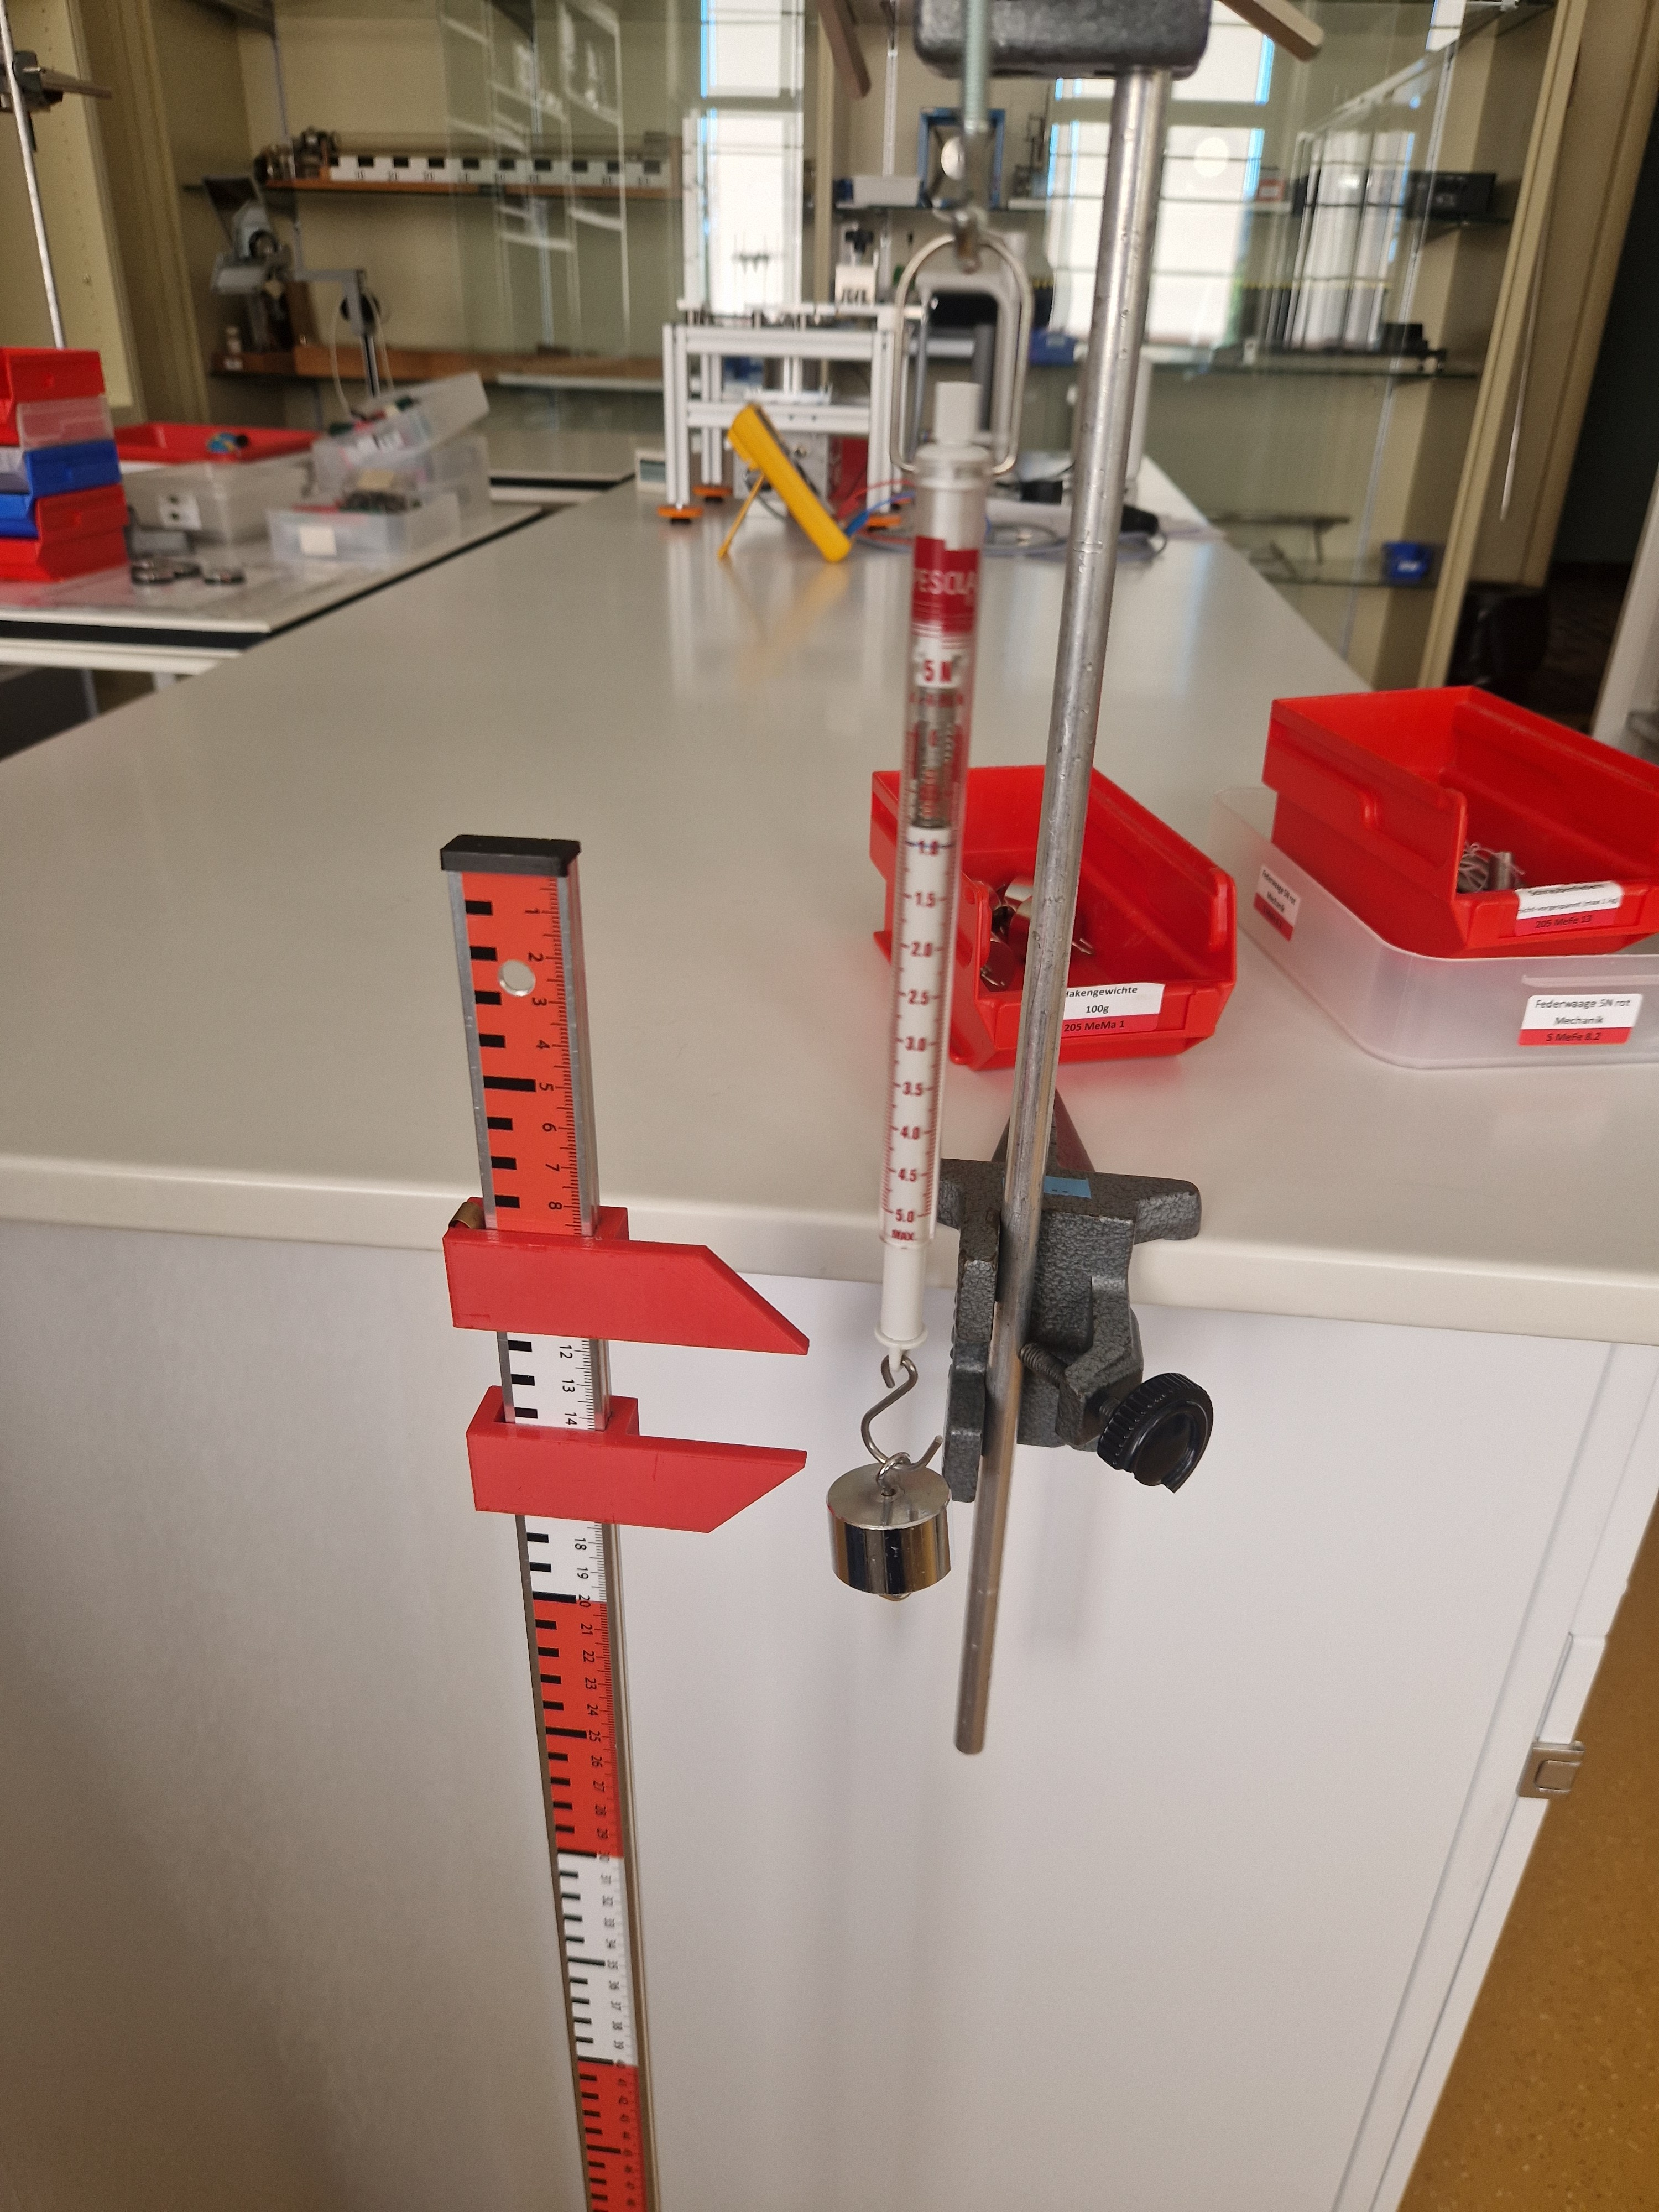
\includegraphics[width=9cm]{Bilder/Federkonstante_Messung_setup.jpg}
\end{center}
{\scriptsize Stationsaufbau: Ein Massstab mit zwei verschiebbaren Köpfen
liegt auf dem Tisch, ein Metallfuss hält die Feder. Der obere Kopf wird beim
Nullpunkt der ungespannten Feder gesetzt; der untere Kopf markiert die
Position bei angehängter Masse. Die rote Federwaage zeigt die
Kraft direkt in Newton an.}

\noindent
\begin{minipage}[c]{1.3cm}
  
\includegraphics[width=1.1cm]{Bilder/excel_logo.jpg}
\end{minipage}%
\begin{minipage}[c]{\dimexpr\linewidth-1.3cm\relax}
\raggedright
Öffnen Sie zu zweit die vorbereitete Excel-Vorlage \texttt{gewichtskraft-\allowbreak
federkraft-\allowbreak messvorlage.xlsx} für Ihre Messwerte.
\end{minipage}

\question\strut

\begin{teilkopf}
Teil 1: Messreihen zur Gewichtskraft in Abhängigkeit von der Längenänderung aufnehmen
\end{teilkopf}
Bauen Sie den Stationsaufbau wie im Foto: Setzen Sie den oberen Kopf des
Massstabs beim Nullpunkt der ungespannten Feder (ohne angehängte Masse).
Hängen Sie nacheinander mehrere Massen an die erste Feder (die stärkere
Feder) und lesen Sie jeweils die Längenänderung $\Delta x$ gegenüber dem
Nullpunkt ab. Berechnen Sie von Hand die Gewichtskraft $F_G=m\cdot g$ jeder
angehängten Masse und tragen Sie Masse, Gewichtskraft und $\Delta x$ in die
Excel-Vorlage ein. Verwenden Sie dabei den exakten Wert des Ortsfaktors
$g=\SI{9.81}{\newton\per\kilogram}$, nicht gerundet auf $10$. Wiederholen
Sie die Messreihe anschliessend mit der Federwaage.
\begin{parts}
  \needspace{3cm}
  \part[5] Welchen Funktionstyp erwarten Sie für den Zusammenhang zwischen
  $F$ und $\Delta x$, und wie äussert sich das im Diagramm, das die
  Excel-Vorlage aus Ihren Werten erstellt? Was entspricht die Steigung der
  Trendlinie physikalisch, und welche Gleichung für den Zusammenhang
  zwischen $F$, $D$ und $\Delta x$ folgt daraus?
  \Antwortraum{5}
  \begin{solution}
  Einen linearen, proportionalen Zusammenhang ($F\sim\Delta x$): Die
  Messpunkte liegen auf einer Ursprungsgeraden (bei korrekt gesetztem
  Nullpunkt). Die Steigung der Trendlinie entspricht der Federkonstante $D$
  der jeweiligen Feder. Da $F$ proportional zu $\Delta x$ ist mit
  Proportionalitätsfaktor $D$, folgt das Hookesche Gesetz:
  \[
    \boxed{F = D\cdot\Delta x}.
  \]
  \end{solution}

  \part[3] Lesen Sie die Federkonstanten $D_1$ (stärkere Feder) und $D_2$
  (Federwaage) aus den beiden Trendliniengleichungen ab (in N/cm) und
  rechnen Sie beide Werte zusätzlich in die SI-Einheit N/m um. Zeigen Sie
  Ihren Rechenweg.
  \Antwortraum{3}
  \begin{solution}
  Individuelle Messwerte: Die abgelesenen Werte $D_1$ und $D_2$ (in N/cm)
  sollten mit den in der Excel-Vorlage angezeigten Trendliniengleichungen
  übereinstimmen. Da $\SI{1}{\centi\meter}=\SI{0.01}{\meter}$ gilt
  $\SI{1}{\newton\per\centi\meter}=\SI{100}{\newton\per\meter}$, zum
  Beispiel bei $D_1=\SI{42}{\newton\per\centi\meter}$:
  \[
    D_1 = \SI{42}{\newton\per\centi\meter} = 42\cdot\SI{100}{\newton\per\meter} = \SI{4200}{\newton\per\meter}
  \]
  (analog für $D_2$ mit dem eigenen Messwert).
  \end{solution}
\end{parts}

\begin{solution}
\noindent
\begin{center}
  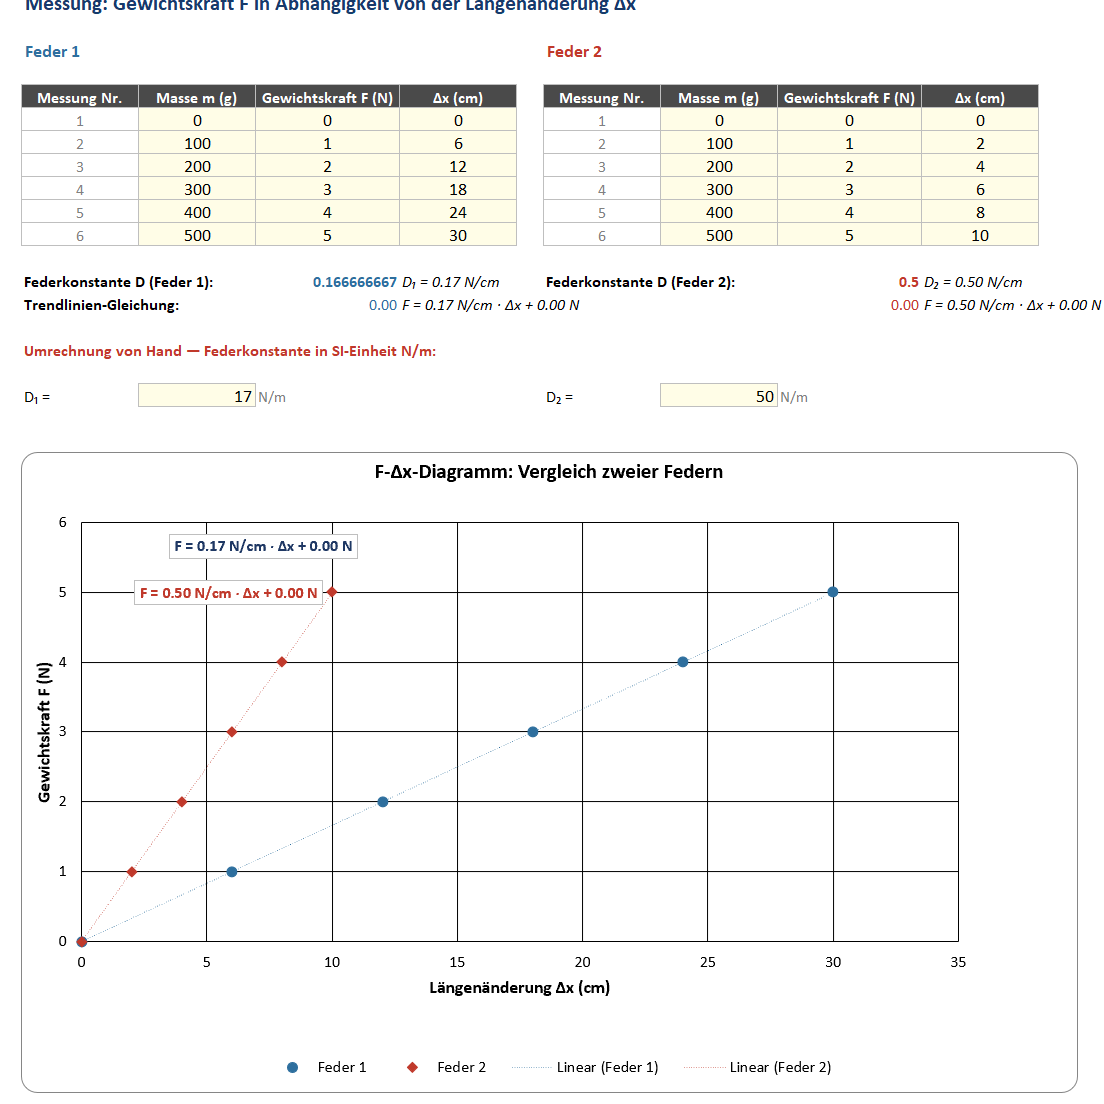
\includegraphics[width=\textwidth]{Bilder/Federexperiment_Excel_Loesung.png}
\end{center}
{\scriptsize Beispiel einer ausgefüllten Excel-Vorlage mit Musterwerten:
Messreihen, Trendliniengleichungen (in N/cm) und die von Hand umgerechneten
Federkonstanten in N/m für beide Federn. Die eigenen Messwerte weichen
davon ab.}
\end{solution}

\question\strut

\begin{teilkopf}
Teil 2: Vergleich der beiden Federn
\end{teilkopf}
\begin{parts}
  \part[4] Welche der beiden Federn ist die stärkere (härtere) Feder? Wie
  erkennt man das direkt an den beiden Trendlinien im gemeinsamen Diagramm,
  und was bedeutet ein grösserer Wert von $D$ für die Auslenkung $\Delta x$
  bei gleicher angehängter Masse?
  \Antwortraum{4}
  \begin{solution}
  Die Feder mit der steileren Trendlinie (dem grösseren Wert von $D$) ist
  die stärkere Feder: Im Diagramm (Gewichtskraft $F$ auf der $y$-Achse,
  Längenänderung $\Delta x$ auf der $x$-Achse) erzeugt dieselbe Auslenkung
  $\Delta x$ bei der stärkeren Feder eine grössere Kraft, was sich als
  steilere Trendlinie zeigt. Für die Auslenkung selbst bedeutet eine
  grössere Federkonstante $D$ umgekehrt, dass bei gleicher Kraft eine
  kleinere Längenänderung $\Delta x$ auftritt ($\Delta x=F/D$).
  \end{solution}

  \needspace{8cm}
  \part[4] Die Federwaage zeigt die Kraft direkt in Newton an, die andere
  (stärkere) Feder ist dagegen unkalibriert. Sie möchten aus dieser
  unkalibrierten Feder selbst eine Federwaage bauen. Zur Verfügung stehen
  Ihnen dafür ein Stift (als Zeiger), mehrere Massen bekannter Grösse und
  ein Gehäuse mit Platz für eine Skala. Beschreiben Sie Schritt für Schritt
  Ihr Vorgehen.
  \Antwortraum{4}
  \begin{solution}
  Zuerst wird die Feder im Gehäuse befestigt und der Stift als Zeiger am
  unteren Ende der Feder angebracht, sodass er sich mit der Feder auf und
  ab bewegt. Ohne angehängte Last markiert man die Position des Zeigers auf
  dem Gehäuse als Nullpunkt ($\SI{0}{\newton}$); eine allfällige
  Vorspannung der Feder wird dabei automatisch mitberücksichtigt.
  Anschliessend hängt man die bekannten Massen nacheinander an, berechnet
  für jede die Gewichtskraft $F_G=m\cdot g$ und markiert die jeweilige
  Zeigerposition mit diesem Kraftwert. So entsteht Schritt für Schritt eine
  Skala in Newton, genau wie beim Kalibrierungsbeispiel mit der
  Schokoladentafel im Arbeitsblatt.
  \end{solution}
\end{parts}

\question\strut

\begin{teilkopf}
Teil 3: Vorhersage und Überprüfung
\end{teilkopf}
Wählen Sie eine Masse, die Sie in Teil~1 noch nicht an der stärkeren Feder
gemessen haben.
\begin{parts}
  \part[3] Berechnen Sie mit Ihrem eigenen Wert von $D_1$ die erwartete
  Längenänderung $\Delta x$ für diese Masse, \emph{bevor} Sie sie anhängen.
  Zeigen Sie Ihren Rechenweg.
  \Antwortraum{3}
  \begin{solution}
  Aus $F=D\cdot\Delta x$ nach $\Delta x$ aufgelöst:
  \[
    \Delta x = \frac{F}{D_1}.
  \]
  Im Gleichgewicht gilt $F=F_G=m\cdot g$ (siehe Kräftediagramm oben),
  eingesetzt:
  \[
    \Delta x = \frac{F_G}{D_1} = \frac{m\cdot g}{D_1}.
  \]
  Individuelle Messwerte: mit der gewählten Masse $m$ und dem eigenen
  $D_1$ ergibt sich die erwartete Längenänderung $\Delta x$.
  \end{solution}

  \part[3] Sie möchten statt für die Erde eine Federwaage bauen, die ein
  Astronaut auf dem Mond benutzen soll (gleiche Feder, gleiches Vorgehen
  wie in Teilaufgabe 2b). Was müssten Sie an Ihrem Vorgehen ändern, damit
  die neue Skala auf dem Mond korrekt funktioniert?
  \Antwortraum{3}
  \begin{solution}
  Die Federkonstante $D$ selbst ändert sich nicht mit dem Ort: Dieselbe
  Auslenkung $\Delta x$ entspricht überall derselben Kraft
  $F=D\cdot\Delta x$. Eine wie in 2b in Newton kalibrierte Federwaage
  funktioniert deshalb unverändert auch auf dem Mond, ohne dass am
  Vorgehen etwas geändert werden müsste. Allerdings landet dieselbe
  Kalibriermasse $m$ dabei an einer anderen Stelle der Skala. Im
  Gleichgewicht gilt für dieselbe Masse $m$:
  \[
    D\cdot\Delta x_{\text{Erde}} = m\cdot g_{\text{Erde}}
    \qquad\text{und}\qquad
    D\cdot\Delta x_{\text{Mond}} = m\cdot g_{\text{Mond}}.
  \]
  Beide Gleichungen nach $m\cdot D$ aufgelöst und gleichgesetzt (bzw. die
  zweite durch die erste geteilt), sodass $m$ und $D$ herausfallen:
  \[
    \frac{\Delta x_{\text{Mond}}}{\Delta x_{\text{Erde}}} = \frac{g_{\text{Mond}}}{g_{\text{Erde}}}
    \quad\Longrightarrow\quad
    \boxed{\Delta x_{\text{Mond}} = \Delta x_{\text{Erde}}\cdot\frac{g_{\text{Mond}}}{g_{\text{Erde}}}}.
  \]
  Da $g_{\text{Mond}}/g_{\text{Erde}}\approx1/6$, dehnt dieselbe
  Kalibriermasse die Feder auf dem Mond nur rund ein Sechstel so weit wie
  auf der Erde. Der Newton-Wert, der an dieser (neuen) Position
  angeschrieben wird, ist aber in beiden Fällen derselbe, nämlich
  $F=m\cdot g_{\text{Mond}}$ bzw. $F=m\cdot g_{\text{Erde}}$ mit dem
  jeweils passenden Ortsfaktor: Die Newton-Skala selbst bleibt also
  richtig, nur die physischen Abstände zwischen den Newton-Markierungen
  auf der Feder unterscheiden sich.

  Anders sieht es aus, wenn die Skala nicht die Kraft in Newton, sondern
  direkt die Masse in Kilogramm anzeigen soll (wie bei einer
  Personenwaage): Dieselbe Masse erzeugt auf dem Mond wegen des kleineren
  Ortsfaktors $g_{\text{Mond}}$ eine rund sechsmal kleinere Gewichtskraft
  und damit eine rund sechsmal kleinere Auslenkung als auf der Erde. Eine
  auf der Erde in Kilogramm geeichte Skala würde auf dem Mond deshalb eine
  viel zu kleine Masse anzeigen.

  An einer bestimmten Position der Skala (also bei fester Auslenkung
  $\Delta x$) wirkt immer dieselbe Federkraft $F=D\cdot\Delta x$,
  unabhängig vom Ort. Die auf der Erde angeschriebene Masse $m_{\text{Erde}}$
  an dieser Position ergibt sich aus $F=m_{\text{Erde}}\cdot g_{\text{Erde}}$,
  die tatsächlich richtige Masse auf dem Mond $m_{\text{Mond}}$ dagegen aus
  $F=m_{\text{Mond}}\cdot g_{\text{Mond}}$. Da $F$ in beiden Gleichungen
  gleich ist, können sie gleichgesetzt werden:
  \[
    m_{\text{Erde}}\cdot g_{\text{Erde}} = m_{\text{Mond}}\cdot g_{\text{Mond}}.
  \]
  Nach $m_{\text{Mond}}$ aufgelöst:
  \[
    \boxed{m_{\text{Mond}} = m_{\text{Erde}}\cdot\frac{g_{\text{Erde}}}{g_{\text{Mond}}}}.
  \]
  Jede Kilogramm-Markierung der Erde-Skala müsste also mit diesem Faktor
  multipliziert werden, um an derselben Position die richtige Masse für
  den Mond anzuzeigen:
  \[
    \frac{g_{\text{Erde}}}{g_{\text{Mond}}} = \frac{\SI{9.81}{\newton\per\kilogram}}{\SI{1.62}{\newton\per\kilogram}} \approx 6.05.
  \]
  Für eine Kilogramm-Skala müsste man also entweder direkt auf dem Mond mit
  bekannten Massen neu kalibrieren, oder die Kilogramm-Markierungen mit
  dieser Formel rechnerisch neu bestimmen.
  \end{solution}
\end{parts}
\end{groupbox}
\end{questions}

\end{document}
